\langsection[subsection]{Handling Dangerous Surfaces}{Проезд по опасным поверхностям}



\begin{langblock}{0.425}
	\begin{eng}
	
	Your chance of falling or being involved in a crash increases whenever you ride across:
	
	\begin{itemize}[noitemsep]
		\item Uneven surfaces or obstacles.
		\item Slippery surfaces.
		\item Railroad tracks.
		\item Grooves and gratings.
	\end{itemize}
	\end{eng}
	\begin{rus}
		
		Вероятность падения или попадания в аварию возрастает при езде по:
		
		\begin{itemize}[noitemsep]
			\item неровному покрытию или препятствиям;
			\item скользкому покрытию;
			\item железнодорожным путям;
			\item канавкам и решеткам.
		\end{itemize}
\end{rus}
\end{langblock}


\langsection[subsubsection]{Uneven Surfaces and Obstacles}{Неровные поверхности и препятствия}



\begin{langblock}{0.425}
	\begin{eng}
	
	Watch for uneven surfaces such as bumps, broken pavement, potholes, or small pieces of highway trash.
	
	Try to avoid obstacles by slowing or going around them. If you must go over the obstacle, first, determine if it is possible. Approach it at as close to a $90^{\circ}$ angle as possible. Look where you want to go to control your path of travel. If you have to ride over the obstacle, you should:
	
	\begin{itemize}[noitemsep]
		\item Slow down as much as possible before contact.
		\item Make sure the motorcycle is straight.
		\item Rise slightly off the seat with your weight on the footpegs to absorb the shock with your knees and elbows, and avoid being thrown off the motorcycle.
		\item Just before contact, roll on the throttle slightly to lighten the front end.
	\end{itemize}
	
	If you ride over an object on the street, pull off the road and check your tires and rims for damage before riding any farther.
	\end{eng}
	\begin{rus}
		
		Обращайте внимание на неровности, такие как бугры, поврежденное дорожное покрытие, выбоины или мелкий мусор на трассе.
		
		Старайтесь обходить препятствия, снижая скорость или объезжая их. Если вам необходимо переехать через препятствие, сначала убедитесь что это возможно. Подъезжайте к нему под углом, максимально приближенным к $90^{\circ}$. Смотрите в том направлении, куда хотите ехать, чтобы контролировать траекторию движения. Для того чтобы переехать через препятствие, вам следует:
		
		\begin{itemize}[noitemsep]
			\item Максимально снизить скорость до момента касания
			\item Убедиться, что мотоцикл находится в вертикальном положении
			\item Слегка привстать с сиденья, перенеся вес на подножки, амортизируйте удар в коленях и локтях чтобы вас не выбросило из седла.
			\item Незадолго до соприкосновения слегка поддайте газу, чтобы разгрузить переднее колесо.
		\end{itemize}
		
		Если вы переехали потенциально опасное препятствие, съедьте с дороги, проверьте шины и диски на наличие повреждений, прежде чем продолжать движение.
\end{rus}
\end{langblock}

\langsection[subsubsection]{Slippery Surfaces}{Скользкие поверхности}


\begin{langblock}{0.425}
	\begin{eng}
	
	
	Motorcycles handle better when ridden on surfaces that permit good traction. Surfaces that provide poor traction include:
	
	\begin{itemize}[noitemsep]
		\item Wet pavement, particularly just after it starts to rain and before surface oil washes to the side of the road.
		\item Gravel roads, or where sand and gravel collect.
		\item Mud, snow, and ice.
		\item Lane markings, steel plates and manhole covers, especially when wet.
	\end{itemize}
	
	
	To ride safely on slippery surfaces:
	
	\begin{itemize}[noitemsep]
		\item Reduce Speed -- Slow down before you get to a slippery surface to lessen your chances of skidding. Your motorcycle needs more distance to stop. And, it is particularly important to reduce speed before entering wet curves.
		\item Avoid Sudden Moves -- Any sudden change in speed or direction can cause a skid. Be as smooth as possible when you speed up, shift gears, turn or brake.
		\item Use Both Brakes -- The front brake is still effective, even on a slippery surface. Squeeze the brake lever gradually to avoid locking the front wheel. Remember, gentle pressure on the rear brake.
		\item The center of a lane can be hazardous when wet. When it starts to rain, ride in the tire tracks left by cars. Often, the left tire track will be the best position, depending on traffic and other road conditions as well.
		\item Watch for oil spots when you put your foot down to stop or park. You may slip and fall.
		\item Dirt and gravel collect along the sides of the road -- especially on curves and ramps leading to and from highways. Be aware of what's on the edge of the road, particularly when making sharp turns and getting on or off freeways at high speeds.
		\item Rain dries and snow melts faster on some sections of a road than on others. Patches of ice tend to crop up in low or shaded areas and on bridges and overpasses. Wet surfaces or wet leaves are just as slippery. Ride on the least slippery portion of the lane and reduce speed.
	\end{itemize}
	
	
	Cautious riders steer clear of roads covered with ice or snow. If you can't avoid a slippery surface, keep your motorcycle straight up and proceed as slowly as possible. If you encounter a large surface so slippery that you must coast, or travel at a walking pace, consider letting your feet skim along the surface. If the motorcycle starts to fall, you can catch yourself. Be sure to keep off the brakes. If possible, squeeze the clutch and coast.  Attempting this maneuver at anything other than the slowest of speeds could prove hazardous.
	\end{eng}
	\begin{rus}
		
		
		Капитан очевидность: мотоцикл лучше едет на поверхности с хорошим сцеплением. К поверхностям с плохим сцеплением относятся:
		
		\begin{itemize}[noitemsep]
			\item Мокрое дорожное покрытие, особенно сразу после начала дождя и до того, как масло со поверхности стечет на обочину.\footnote{Зависит от интенсивности дождя. Первые час-два дорога особенно скользкая. Грязь набухла, стала склизкой, но еще не успела стечь в сторону обочины.}
			\item Гравийные дороги или участки, где скапливаются песок и гравий.
			\item Грязь, снег и лед.
			\item Разметка, стальные пластины и крышки люков, особенно когда они мокрые.
		\end{itemize}
		
		
		Чтобы безопасно ездить по скользким поверхностям:
		
		\begin{itemize}[noitemsep]
			\item Снизьте скорость "--- замедлитесь до въезда на скользкий участок, чтобы уменьшить вероятность заноса. Вашему мотоциклу для остановки потребуется больший тормозной путь. Кроме того, особенно важно снизить скорость перед входом в мокрые повороты.
			\item Избегайте резких маневров "--- Любое резкое изменение скорости или направления может привести к заносу. Старайтесь действовать как можно плавнее при ускорении, переключении передач, поворотах или торможении.
			\item Используйте оба тормоза "--- Передний тормоз остается эффективным даже на скользкой поверхности. Нажимайте на тормозной рычаг плавно, чтобы не заблокировать переднее колесо. Помните: на задний тормоз следует нажимать мягко.
			\item Центральная часть полосы может быть опаснее на мокрой дороге. Когда начинается дождь, езжайте по колеям, оставленным автомобилями. Левая колея лучший выбор, но многое зависит от интенсивности движения и других дорожных условий.
			\item Следите за масляными пятнами, когда ставите ногу на землю, чтобы остановиться на светофоре или припарковаться. Вы можете поскользнуться и упасть.
			\item Грязь и гравий скапливаются по бокам дороги "--- особенно на поворотах и съездах, ведущих к автомагистралям и с них. Следите за тем, что находится на краю дороги, особенно при выполнении резких поворотов и въезде или съезде с автомагистралей на высокой скорости.
			\item На некоторых участках дороги дождь высыхает, а снег тает быстрее, чем на других. Пятна льда обычно появляются в низинах или затененных местах, а также на мостах и эстакадах. Мокрые поверхности или мокрые листья так же скользкие. Двигайтесь по наименее скользкой части полосы движения и снизьте скорость.
		\end{itemize}
		
		
		Разумные мотоциклисты не выезжают на обледенелые или заснеженные дороги. Если по-другому никак и вам надо проехать по скользкой поверхности, держите мотоцикл ровно и двигайтесь как можно медленнее. Если вы столкнулись с большим участком, настолько скользким, что вам приходится двигаться накатом или ехать со скоростью пешехода, опустите ноги, позволяя им скользить по земле. Если мотоцикл начнет падать, вы сможете удержать его. Обязательно держитесь подальше от тормозов. По возможности выжмите сцепление и двигайтесь накатом.  Попытка выполнить этот маневр на любой скорости, кроме самой низкой, может оказаться фатальной.
\end{rus}
\end{langblock}


\langsection[subsubsection]{Railroad Tracks, Trolley Tracks and Pavement Seams}{Железнодорожные пути, троллейбусные колеи и швы}

\begin{figure}[htbp]
	\begin{subfigure}{0.45\textwidth}	
		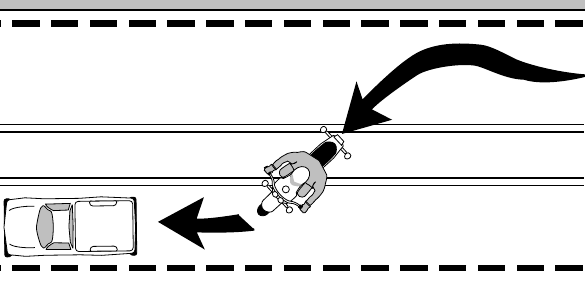
\includegraphics[width=0.95\textwidth, frame]{images/crosstrac_3.png}
		\caption{Parallel tracks-right}
		\label{fig:crosstrac_3}
	\end{subfigure}
	\hspace*{\fill}
	\begin{subfigure}{0.45\textwidth}	
		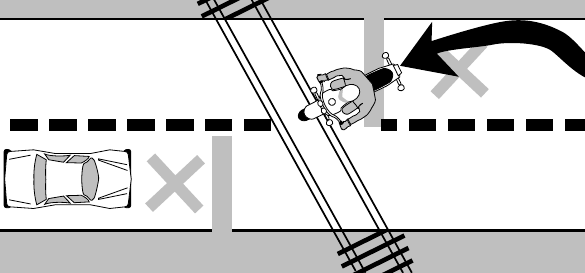
\includegraphics[width=0.95\textwidth, frame]{images/crosstrac_2w.png}
		\caption{Parallel tracks-wrong???}
		\label{fig:crosstrac_2wwww}
	\end{subfigure}
	
	\begin{subfigure}{0.45\textwidth}
		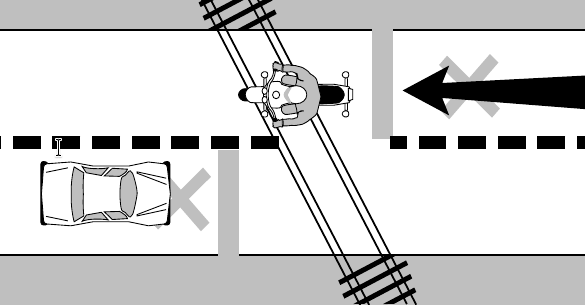
\includegraphics[width=0.95\textwidth, frame]{images/crosstrac_1.png}
		\caption{Crosstracks-right}
		\label{fig:crosstrac_1}
	\end{subfigure}
	\hspace*{\fill}
	\begin{subfigure}{0.45\textwidth}	
		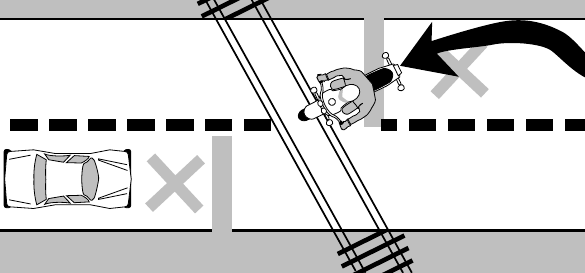
\includegraphics[width=0.95\textwidth, frame]{images/crosstrac_2w.png}
		\caption{Crosstracks-wrong}
		\label{fig:crosstrac_2w}
	\end{subfigure}
	
	\caption{Tracks}
\end{figure}


\begin{langblock}{0.425}
	\begin{eng}
	
	Usually it is safer to ride straight within your lane to cross tracks.  Turning to take tracks head-on (at a $90^{\circ}$ angle) can be more dangerous -- your path may carry you into another lane of traffic.
	
	For track and road seams that run parallel to your course, move far enough away from tracks, ruts, or pavement seams to cross at an angle of at least $45^{\circ}$. Then, make a deliberate turn. Edging across could catch your tires and throw you off balance.
	\end{eng}
	\begin{rus}
		
		Переезжая ЖД пути, обычно безопаснее ехать просто прямо, в пределах своей полосы. Выворачиваясь так чтобы переехать рельсы под прямым углом ($90^{\circ}$) может быть более опасным "--- вас может вынести на другую или встречную полосу движения.
		
		Если колея и шов дорожного покрытия идет параллельно вашему курсу, отступите на достаточное расстояние, а потом вырулите так чтобы пересечь их под углом не менее $45^{\circ}$. Пересечение под острым углом может зацепить шину за край и выбросить вас из седла.\footnote{Вообще люди делятся на два типа: те кто еще не в курсе, что нельзя заезжать на препятствие под острым углом и тех, кто фанатично пытается переехать все подряд строго под $90^{\circ}$. На мото нет ничего страшнее, чем въехать в параллельную канавку, а так же положить мото набок из-за неудачного угла заезда на бордюр. Это приходит с опытом. Угол должен быть тупым, но дальше детали и частности.}
\end{rus}
\end{langblock}









\langsection[subsubsection]{Grooves and Gratings}{Пазы и решетки}

\begin{figure}[htbp]
	\begin{subfigure}{0.45\textwidth}	
		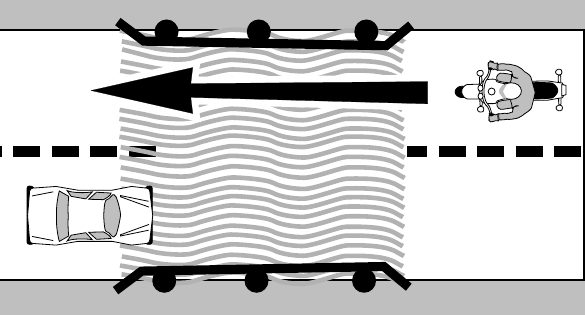
\includegraphics[width=0.95\textwidth, frame]{images/gcros_1.png}
		\caption{Gratecrossings-right}
		\label{fig:gcros_1}
	\end{subfigure}
	\hspace*{\fill}
	\begin{subfigure}{0.45\textwidth}	
		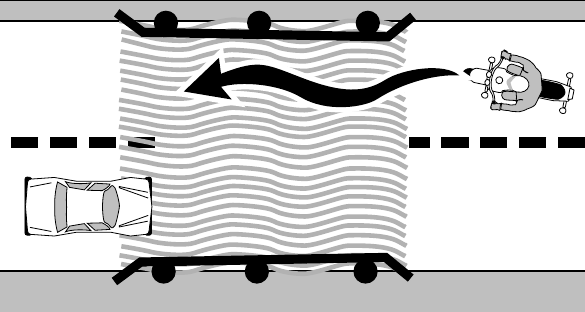
\includegraphics[width=0.95\textwidth, frame]{images/gcros_2w.png}
		\caption{Gratecrossings-wrong}
		\label{fig:gcros_2w}
	\end{subfigure}
		
	\caption{Grooves and Gratings}
\end{figure}


\begin{langblock}{0.425}
	\begin{eng}
	
	Riding over rain grooves or bridge gratings may cause a motorcycle to weave. The uneasy, wandering feeling is generally not hazardous. Relax, maintain a steady speed and ride straight across. Crossing at an angle forces riders to zigzag to stay in the lane. The zigzag is far more hazardous than the wandering feeling.
	\end{eng}
	\begin{rus}
		
		Проезд по продольным водоотводным канавкам (нарезные борозды) или решеткам мостов (стальная решетчатая палуба моста) может привести к вилянию мотоцикла. Это ощущение неустойчивости и «блуждания» обычно не представляет опасности. Расслабьтесь, поддерживайте постоянную скорость и езжайте прямо. Попытка поймать правильную траекторию вынуждает мотоциклистов ехать зигзагом. Зигзагообразная езда гораздо опаснее, чем ощущение «рысканья».
\end{rus}
\end{langblock}








